\documentclass{article}
\topmargin -0.5in \oddsidemargin -0.25in \textheight 9in
\textwidth 6.5in
\usepackage{graphics}
\usepackage{graphicx}
\usepackage{forest}
\usepackage{tikz}
\usepackage{amsmath}
\usepackage{amssymb}


\newcommand{\shrink}[1]{}

\begin{document}
{\bf ICS 271}

{\bf Fall 2016}

{\bf Student ID : 26642334}

{\bf Student Name: Yu Guo}

{\bf Instructor : Kalev Kask}

{\bf Homework Assignment 2}

{\bf Due Tuesday, 10/18}




\begin{enumerate}

% 1.
\item
\begin{enumerate}
  \item Step 1

  
\includegraphics[width=0.6\textwidth]{figure/Slide1.PNG}

  \item Step 2
  
  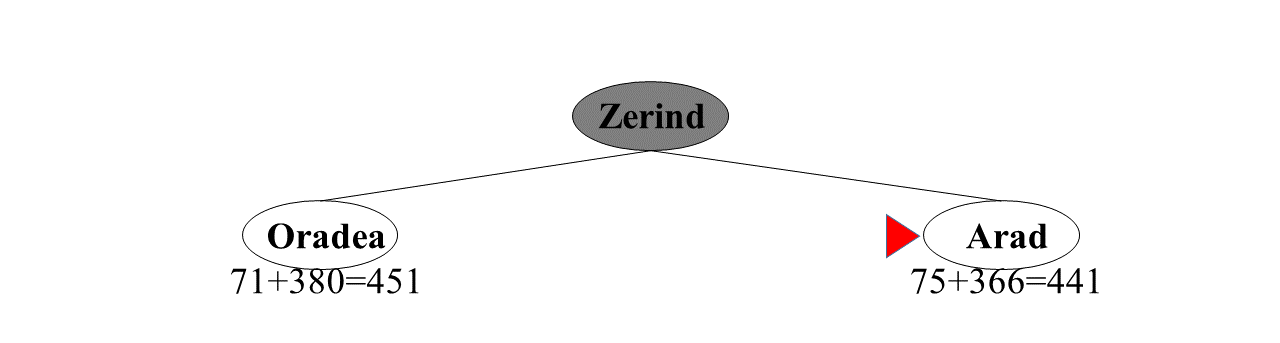
\includegraphics[width=0.6\textwidth]{figure/Slide2.PNG}

  \item Step 3
  
  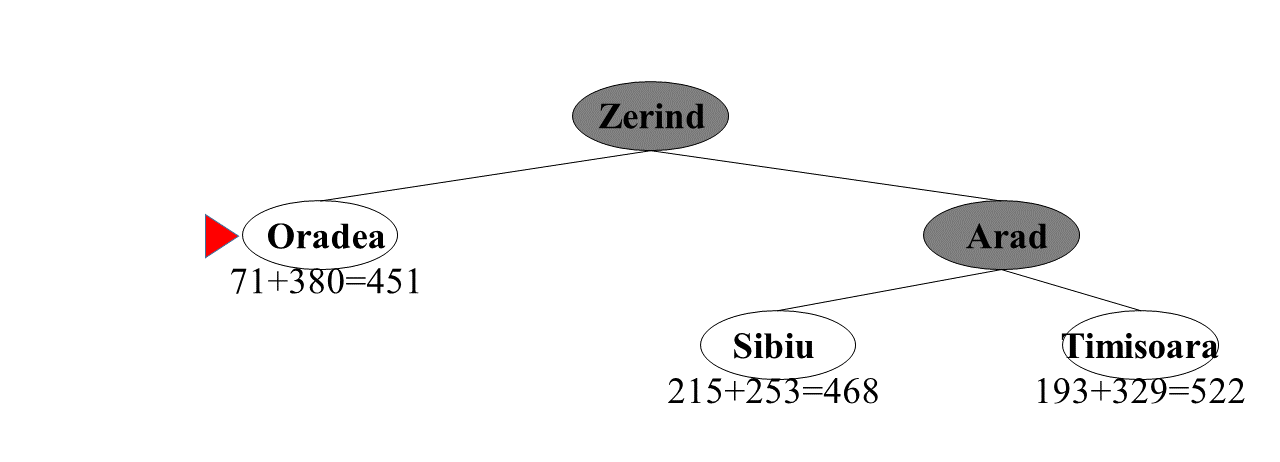
\includegraphics[width=0.6\textwidth]{figure/Slide3.PNG}

  \item Step 4
  
  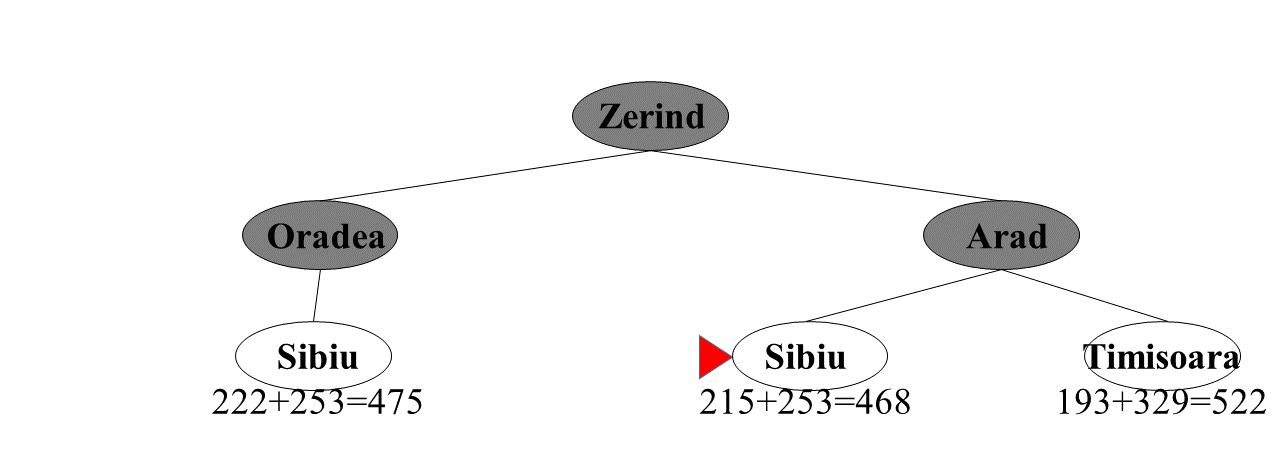
\includegraphics[width=0.6\textwidth]{figure/Slide4.PNG}

  \item Step 5
  
  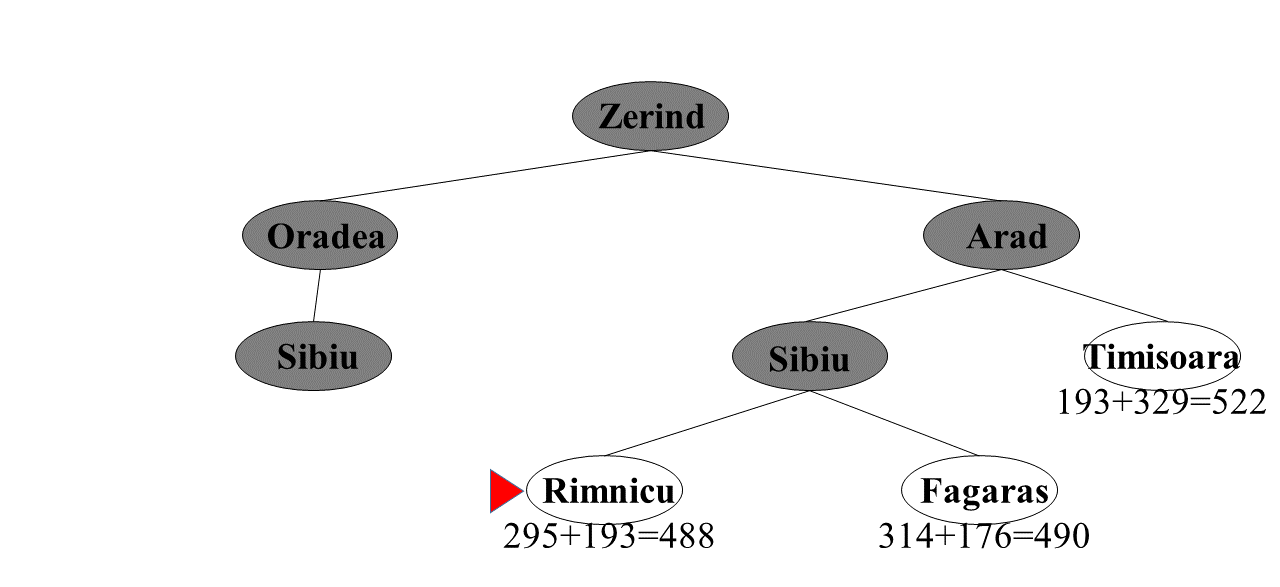
\includegraphics[width=0.6\textwidth]{figure/Slide5.PNG}

  \item Step 6
  
  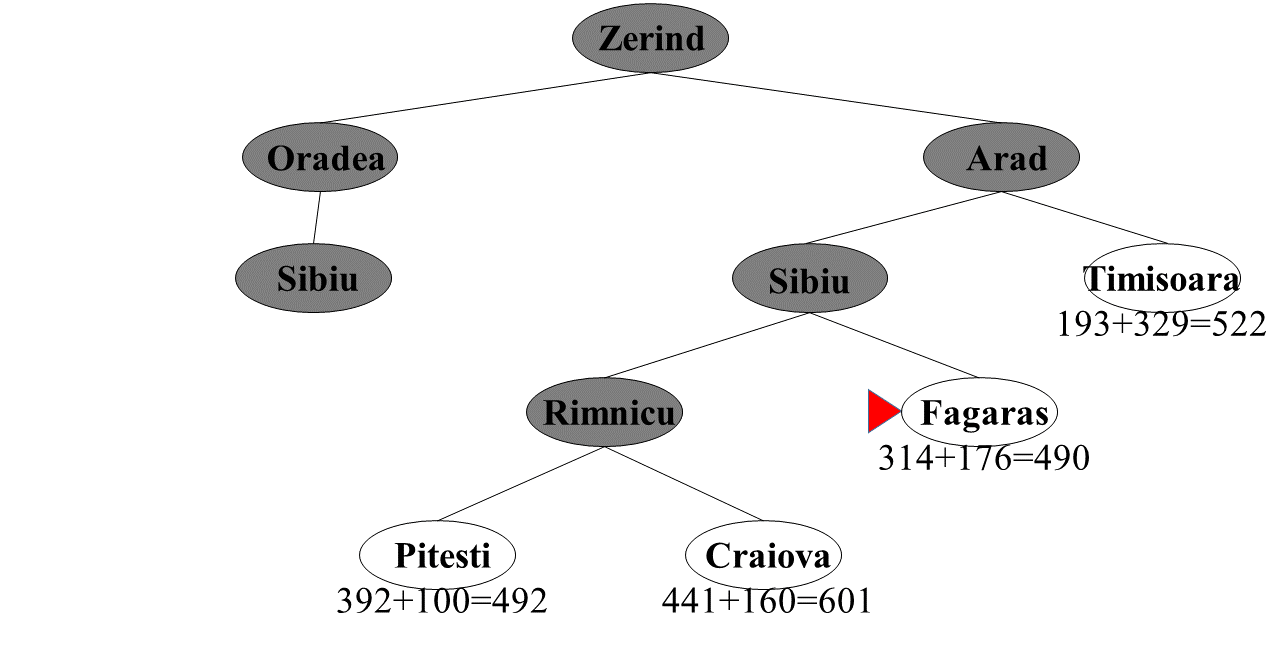
\includegraphics[width=0.6\textwidth]{figure/Slide6.PNG}

  \item Step 7
  
  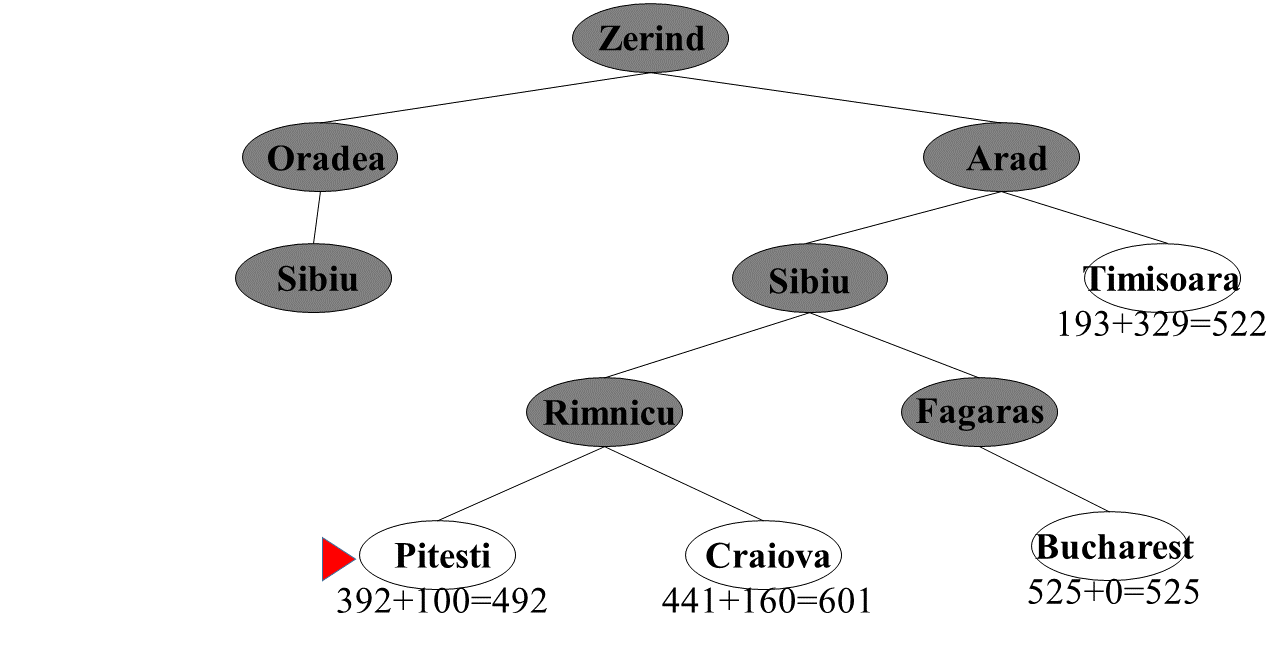
\includegraphics[width=0.6\textwidth]{figure/Slide7.PNG}

  \item Step 8
  
  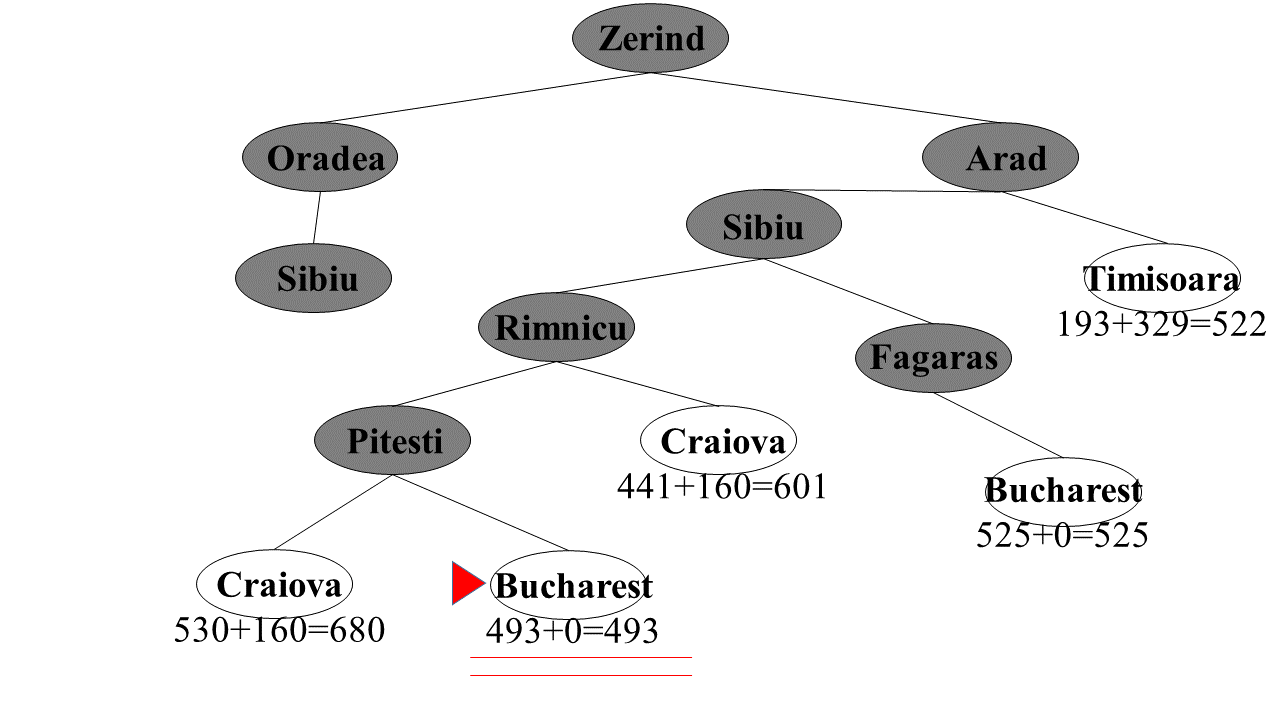
\includegraphics[width=0.6\textwidth]{figure/Slide8.PNG}


\end{enumerate}


% 2.
\item

\begin{enumerate}
  \item
  \begin{equation}
  \begin{aligned}
  f(n+1) &= g(n+1) \\
         &= g(n) + c(n,n+1) \\
         &\geqslant g(n) \\
         &\geqslant f(n)  
  \end{aligned}
  \end{equation}


  \item
  \begin{equation}
  \begin{aligned}
  h(n) &= max(h_1(n),h_2(n)) \\
       &\leqslant max(h_1(n') + c(n,n'), h_2(n') + c(n,n')) \\
       &\leqslant max(h_1(n'),h_2(n')) + c(n,n') \\
       &\leqslant h(n') + c(n,n')  
  \end{aligned}
  \end{equation}

  \item
  $h$ is consistent, so $h(n) \leqslant h(n') + c(n,n')$. Also we have $h(n^{goal}) = 0$. 
  Then,
  \begin{equation}
  \begin{aligned}
  h(n^{goal-1}) &\leqslant h(n^{goal}) + c(n^{goal-1},n^{goal}) \\
                &\leqslant c(n^{goal-1},n^{goal}) \\
  h(n^{goal-2}) &\leqslant h(n^{goal-1}) + c(n^{goal-2},n^{goal-1}) \\
                &\leqslant c(n^{goal-2},n^{goal}) \\
                &. \\
                &. \\
                &. \\                  
  h(n^{goal-i}) &\leqslant h(n^{goal-i}) + c(n^{goal-i-1},n^{goal-i}) \\
                &\leqslant c(n^{goal-i},n^{goal})
  \end{aligned}
  \end{equation}
  For any node, it's admissible since it always underestimates the path cost to the goal state.

  \item
  \begin{equation}
  \begin{aligned}
  f(n) &= g(n) + h(n) \\
       &\leqslant g(n) + h(n') + c(n,n') \\  
       &\leqslant g(n) + c(n,n') + h(n') \\
       &\leqslant g(n') + h(n') \\
       &\leqslant f(n')       
  \end{aligned}
  \end{equation} 
  $f(n)$ is always increasing, once a node has been visited, it cannot be visited again at a smaller cost. 

  \item
  For node $h_1(n) > h_2(n)$, we have $f_1(n) > f_2(n)$. 
  If node $n$ has the smallest value in opened nodes, the same node is expanded by both heuristics.
  If exist a node $n'$ in opened nodes, that $f_1(n) > f_1(n')$ and $f_2(n) < f_2(n')$, we should choose $n'$ for $f_1$ but keep $n$ for $f_2$. If $n'$ leed to the goal, heuristic $h_2$ would need more steps to the goal. In this way, $A^*$ with $h_1$ always expands less nodes than $A^*$ with $h_2$.


\end{enumerate}


% 3.
\item

If $0 \leqslant \omega \leqslant 1$, Complete

If $0 \leqslant \omega \leqslant 1$, Optimal

If $\omega = 0$, $f(n)=2g(n)$, Uninformed best-first search

If $\omega = 1$, $f(n)=g(n)+h(n)$, $A^*$ search

If $\omega = 2$, $f(n)=2h(n)$, Greedy best-first search

% 4.
\item
Yes. When we compute the cost($g(n)$) of one node, if $g(n) \geqslant f_U$, we can close this node because this path would cost more than the exist path $U$.

% 5.
\item
When a goal node has been found, it only can say that it's one solution but not the optimal solution.

For example, let's look at Question 1 of this homework. In Step 7, it's the first time we reached the goal city Bucharest with cost of 525. But this is not the lowest cost of path. The lowest cost should be in Step 8, and the cost is 493, smaller than 525.

\end{enumerate}

\end{document}